\documentclass[conference]{IEEEtran}
\IEEEoverridecommandlockouts
% The preceding line is only needed to identify funding in the first footnote. If that is unneeded, please comment it out.
\usepackage{cite}
\usepackage{amsmath,amssymb,amsfonts}
\usepackage{algorithmic}
\usepackage{graphicx}
\usepackage{textcomp}
\usepackage{xcolor}
\usepackage{hyperref} 
\def\BibTeX{{\rm B\kern-.05em{\sc i\kern-.025em b}\kern-.08em
    T\kern-.1667em\lower.7ex\hbox{E}\kern-.125emX}}
\begin{document}

\title{Federated TimeVQVAE Anomaly Detection:\\
Prior Sharing Requires an Aligned Tokenizer}

\author{\IEEEauthorblockN{1\textsuperscript{st} Leonardo Schiavo}
\IEEEauthorblockA{\textit{Departamento de Sistemas Inform\'aticos} \\
\textit{Universidad Polit\'ecnica de Madrid}\\
Madrid, Spain \\
leonardo.schiavo@upm.es}
\and
\IEEEauthorblockN{2\textsuperscript{nd} Donato Cerciello}
\IEEEauthorblockA{\textit{Departamento de Sistemas Inform\'aticos} \\
\textit{Universidad Polit\'ecnica de Madrid}\\
Madrid, Spain \\
donato.cerciello@upm.es}
\and
\IEEEauthorblockN{3\textsuperscript{rd} \'Angel Panizo-Lledot}
\IEEEauthorblockA{\textit{Departamento de Sistemas Inform\'aticos} \\
\textit{Universidad Polit\'ecnica de Madrid}\\
Madrid, Spain \\
angel.panizo@upm.es}
\and
\IEEEauthorblockN{4\textsuperscript{th} Javier Huertas Tato}
\IEEEauthorblockA{\textit{Departamento de Sistemas Inform\'aticos} \\
\textit{Universidad Polit\'ecnica de Madrid}\\
Madrid, Spain \\
javier.huertas.tato@upm.es}
\and
\IEEEauthorblockN{5\textsuperscript{th} Stefano Izzo}
\IEEEauthorblockA{\textit{Department of Mathematics and Applications ``R. Caccioppoli''} \\
\textit{University of Naples Federico II}\\
Naples, Italy \\
stefano.izzo@unina.it}
\and
\IEEEauthorblockN{6\textsuperscript{th} Fabio Giampaolo}
\IEEEauthorblockA{\textit{Department of Mathematics and Applications ``R. Caccioppoli''} \\
\textit{University of Naples Federico II}\\
Naples, Italy \\
fabio.giampaolo@unina.it}
\and
\IEEEauthorblockN{7\textsuperscript{th} David Camacho}
\IEEEauthorblockA{\textit{Departamento de Sistemas Inform\'aticos} \\
\textit{Universidad Polit\'ecnica de Madrid}\\
Madrid, Spain \\
david.camacho@upm.es}
}

\maketitle

\begin{abstract}
Time series anomaly detection is often carried out by parties that cannot pool their raw data,
which makes federated training attractive. We ask what should be shared when the detector is a
two-stage generative model: TimeVQVAE-AD first learns a discrete tokenizer of the signal, and then
a prior over the resulting tokens. We find that the two stages cannot be federated independently.
Sharing the prior helps only once the clients' tokenizers have been aligned by averaging their
encoders, and the identical change brings nothing when they have not been, because the prior is
indexed by token identity and unaligned clients use those identities differently. We evaluate this
on the UCR anomaly archive, with every series split across five clients, on ten series used for
development and on fifty further series drawn at random in advance. The federated model improves
over local training in the ranking of anomalous timesteps, and on the archive's own localization
metric it matches pooled training on most series -- a metric on which pooled training, which sees
all the data, does not separate from local training either. We also describe a case in which averaging spreads
one client's false alarm to every client, and show that combining the local models' scores instead
of their weights avoids it.
\end{abstract}

\begin{IEEEkeywords}
federated learning, time series anomaly detection, vector quantization, generative models,
model aggregation
\end{IEEEkeywords}

\section{Introduction}

Time series anomaly detection~\cite{blazquezgarcia2022review,schmidl2022anomaly} is often
performed in distributed settings, where sensors, machines, or organizations collect data
independently and cannot share their raw observations~\cite{zhu2022fedexdnn,xu2024pefad}.
Federated learning (FL)~\cite{mcmahan2017federated} offers a natural way to exploit data
across participants without centralizing their raw series. On the UCR anomaly
archive~\cite{wu2023ucr}, our experiments confirm that such collaboration can be valuable:
whenever the methods can be distinguished, pooled training outperforms the average client,
although not necessarily the best local model.

We study how this collaboration can be realized for
TimeVQVAE-AD~\cite{lee2024timevqvaead}, a two-stage generative anomaly detector composed of a
VQ-VAE~\cite{van2017neural} tokenizer and a masked prior over the resulting discrete
tokens~\cite{lee2023timevqvae}. Its two-stage structure raises a question that is less
explicit in conventional end-to-end detectors: which components should be shared across
clients, and how should federation of the tokenizer and the prior be coordinated?

Our experiments show that these decisions cannot be made independently. Sharing the codebook
alone can underperform purely local training, while federating the encoder, pooling batch
normalization (BN) statistics, and aggregating the codebook through sufficient statistics
does not improve over the local baseline when the prior remains local. The strongest
federated configuration instead combines encoder FedAvg~\cite{mcmahan2017federated}, pooled
BN statistics, sufficient-statistics codebook aggregation, and a mostly shared prior, while
keeping the channel embedding, output bias, and decoder local.
On the ten development series this configuration takes the archive's accuracy from $0.40$, $0.80$
and $0.20$ to $1.00$ on the three series where federation and pooling separate at all, matching
centralized training exactly, and drops from $0.20$ to $0.00$ on a fourth, \texttt{ucr\_170},
which we analyze as a failure case. On a pre-registered random sample of fifty further series it
improves the ranking of anomalous timesteps over local training on thirty-two of forty-eight
($p=0.029$ in AUPRC) and matches centralized training on the archive's own accuracy metric on
thirty-seven of forty-eight. On that metric the pre-registered primary endpoint does not reach
significance for any contrast, centralized training included, so what the sample establishes is
parity with the pooled upper bound rather than a demonstrated gain in localization. We report the
endpoint we fixed in advance, and we do not claim the stronger reading.

Matched ablations show that the improvement comes from prior sharing, but only after the
token representation has been aligned across clients. This is consistent with the general
observation that parameter averaging requires compatible internal representations
~\cite{entezari2022permutation,ainsworth2023gitrebasin,wang2020fedma}: for a discrete
generative model, prior parameters can be meaningfully shared only when token indices have
common semantics and clients map windows to those tokens consistently. Tokenizer and prior
federation must therefore be coordinated.

Our contributions are:

\begin{enumerate}

\item \textbf{A coordinated federation strategy for tokenizer-based generative anomaly
detectors.}
We show experimentally that sharing the prior becomes beneficial only after aligning the
token representation, and obtain the strongest federated configuration by jointly
coordinating encoder, BN statistics, codebook, and prior federation.

\item \textbf{A characterization of a failure mode of weight-space aggregation and a
function-space alternative.}
On cases such as \texttt{ucr\_170}, federated aggregation can propagate client-specific
false alarms across models. Averaging the z-normalized anomaly scores
~\cite{kriegel2011unifying} of the unaggregated local models instead closes most of the AUPRC
gap to centralized training, forming the ensemble in function space
~\cite{aggarwal2015outlierensembles,lin2020feddf} rather than weight space.

\end{enumerate}

\section{Related Work}

\subsection{Federated Learning}

Federated learning (FL) lets multiple clients train a shared model while their data stay
local~\cite{kairouz2021advances}, with FedAvg as the standard reference
point~\cite{mcmahan2017federated}. Parameter averaging is brittle when local models drift
apart, and the remedies act at three different places: on the local objective, as in FedProx,
which adds a proximal term~\cite{li2020fedprox}; on the local update, as in SCAFFOLD, which
corrects client drift with control variates~\cite{karimireddy2020scaffold}; or on the server,
which can treat the aggregate as a gradient and apply an adaptive
optimizer~\cite{reddi2021adaptive}. FedMA instead matches internal units before averaging
them~\cite{wang2020fedma}. A second line shares only part of the model and keeps
the rest local, a global body with personal heads~\cite{arivazhagan2019fedper,collins2021fedrep},
or the mirror image arrangement with local representations and a global
head~\cite{liang2020lgfedavg}. What matters is therefore not only \emph{what} is shared,
but \emph{how} it is aggregated and \emph{which} part is left local.

\subsection{Federated Time series Anomaly Detection}

Federated methods for time series anomaly detection (TSAD) collaborate without transferring
raw series. Fed-ExDNN learns a per device \emph{exemplar} module of normal patterns and
aggregates the exemplar parameters at the server through constrained clustering, aligning
them before they are averaged~\cite{zhu2022fedexdnn}; PeFAD reduces the communicated
parameters by parameter efficiently adapting a pre trained language model, relying on a
shared synthetic dataset for distillation~\cite{xu2024pefad}. In both cases the aggregated
representation is the \emph{terminal} one, read directly by a scoring function. To our
knowledge, no federated TSAD work addresses a pipeline in which a discrete tokenizer produces
the symbols consumed by a second, generative prior.

\subsection{VQ-VAE and Discrete Tokenization of Time Series}

VQ-VAE introduces a discrete latent representation built on a learned codebook, over which a
prior on the codes is fitted in a second stage~\cite{van2017neural}. TimeVQVAE carries this
principle to time series, combining quantization in the time--frequency domain with a
Transformer prior~\cite{lee2023timevqvae}; TimeVQVAE-AD reuses the same structure for
anomaly detection, scoring a window by the negative log-likelihood its prior assigns to the
window's tokens~\cite{lee2024timevqvaead}. Tokenizer and prior are thus coupled by
construction: the second is a model of the first one's output.

\subsection{Federated Sharing of Representations and Codebooks}

A further line transfers knowledge without averaging full weight vectors: k-FED studies
one shot federated clustering of centroids~\cite{dennis2021kfed}, FedProto shares class
prototypes~\cite{tan2022fedproto}, and Orchestra builds globally consistent representations
through distributed clustering~\cite{lubana2022orchestra}. These are the closest analogues
to sharing a codebook, but centroids and prototypes are not a discrete vocabulary read by a
downstream model: aligning them improves the quality of the aggregate, not its
well definedness. That dependency is what we study. When the vocabulary is itself the object
of federation, cross client alignment becomes a precondition for sharing the prior to be
well posed at all; we measure its effect on detection, compare codebook sharing strategies,
and characterize the cases in which collaboration fails to recover the local baseline.




\section{Background: TimeVQVAE-AD}
\label{sec:background}

We summarize the detector that we federate, following~\cite{lee2024timevqvaead}, and fix the
notation used in the rest of the paper. Throughout, a \emph{client} owns a set of windows of a
univariate series and never shares them.

\subsection{Two-stage training}

TimeVQVAE-AD inherits the two-stage scheme of VQ-VAE~\cite{van2017neural}, instantiated for time
series by TimeVQVAE~\cite{lee2023timevqvae}. In the first stage, a window $x \in \mathbb{R}^{T}$
is moved to the time--frequency domain by a short-time Fourier transform and then encoded and
quantized,
\begin{equation}
  z_q = \mathrm{VQ}\bigl(E(\mathrm{STFT}(x))\bigr), \qquad z_q \in \mathbb{R}^{D \times H \times W},
  \label{eq:tokenize}
\end{equation}
where $H$ is the number of frequency bands, $W$ the latent temporal length, and $D$ the latent
dimension. The encoder $E$, the vector quantizer $\mathrm{VQ}$ with codebook
$\mathcal{C} = \{e_k\}_{k=1}^{K}$, and the decoder $\mathrm{Dec}$ are trained by minimizing the
reconstruction error
\begin{equation}
  \mathbb{E}_{x \sim \mathcal{X}}\bigl\|\, x - \mathrm{Dec}\bigl(\mathrm{VQ}(E(\mathrm{STFT}(x)))\bigr) \bigr\|.
  \label{eq:stage1}
\end{equation}
We write $s \in \{1,\dots,K\}^{H \times W}$ for the grid of codebook indices of $z_q$ and call its
entries \emph{tokens}.

In the second stage, $E$ and $\mathrm{Dec}$ are frozen and a bidirectional transformer, a MaskGIT
prior~\cite{chang2022maskgit}, learns the prior $p_\theta(s)$ over that grid by masked modeling,
maximizing
\begin{equation}
  \mathbb{E}_{x \sim \mathcal{X}}\bigl[\, p_\theta(s \mid s_M) \,\bigr],
  \label{eq:stage2}
\end{equation}
where $s_M$ replaces a uniformly random subset of the tokens by a \texttt{[MASK]} symbol. The two
stages thus stand in a producer--consumer relation: the prior is a categorical model \emph{over the
indices} emitted by the first stage, and the rows of its output layer are indexed by that stage's
codebook.

The convolutional kernels of the encoder and decoder are frequency independent, preserving the temporal and frequency semantics of $\mathrm{STFT}(x)$ in $s$. Each token $s_{h,w}$ therefore localizes a specific time and frequency region, allowing anomaly scores to be mapped back to the original series.

\subsection{Anomaly score}

Detection happens at inference time only; no anomaly label is used at any stage of training. Given
a window, its tokens are computed once and a masking window slides along the temporal axis of the
latent grid. For a latent step $w$ and an odd latent-window size $\kappa = 2\alpha + 1$, the tokens
in the columns $[w-\alpha,\, w+\alpha]$ are masked \emph{across all frequency bands}, and the score
of that step is the mean negative log-likelihood the prior assigns to the true tokens of the masked
region,
\begin{equation}
  a_w = \mathbb{E}\bigl[-\log p_\theta\bigl(s_{:,\,w-\alpha:w+\alpha} \mid s_{M(:,\,w-\alpha:w+\alpha)}\bigr)\bigr].
  \label{eq:aw}
\end{equation}
Scoring the whole masked region rather than its central column alone is deliberate: neighboring
latent steps share receptive field through the convolutional encoder, and the authors report the
regional variant to be the more robust of the two.

The latent window size is not a single choice. It is derived as $\kappa = \mathrm{odd}(r\,W)$ from a
set of rates $r \in \{0.1, 0.3, 0.5\}$, spanning narrow to wide contexts, and the resulting maps are
summed: a short-range anomaly is captured at a small $\kappa$ and a trend shift at a large one,
without any retraining. The sum is then averaged over the frequency dimension, mapped back to the
data space by nearest-neighbor interpolation, and accumulated over the rolling windows that cover
the series, yielding a per-timestep score $\bar{a}$. A final \emph{impulse} term
\begin{equation}
  a_{\text{final}} = \tfrac{1}{2}\bigl(\bar{a} + \mathrm{MA}_T(\bar{a})\bigr)
  \label{eq:afinal}
\end{equation}
averages $\bar{a}$ with its centered moving average of length $T$, so that a long anomaly of
moderate amplitude is not out ranked by a short spike, the argmax over $\bar{a}$ alone is blind to
duration. The anomaly score is computed from the prior alone: it is the likelihood the prior assigns to the
observed tokens, and no reconstruction of the input takes part in it. Every federation choice that
touches the tokenizer therefore reaches detection only through the token grid the prior consumes
and through the vocabulary it predicts. Second, the decoder plays no part in the score, so keeping
it local costs nothing in detection terms.

\subsection{Configuration inherited from the original method}

Two settings are treated here as part of the detector rather than as hyperparameters, because the
original method states them as such~\cite{lee2024timevqvaead}: the window length is $T = 2P$, twice
the period of the series, with $P$ taken from the manual per-dataset measurements released by the
authors, and each input window is z-normalized before the STFT. We likewise keep
the frequency resolution of the original ($\texttt{n\_fft} = 4$, i.e.\ $H = 3$ bands) and its latent
temporal resolution (downsampled width $32$); the remaining capacity settings are ours, and are
stated with the experimental protocol.

Finally, the coupling between the two stages restricts what federation can even mean here. A token
is a pointer into a codebook, so averaging prior parameters across clients presupposes that index
$k$ denotes the same codeword on every client; and since the index is produced by $E$ and
$\mathrm{VQ}$ jointly, it further presupposes that clients agree on \emph{which} windows map to $k$.
Sharing a dictionary secures the first condition and not the second. This is the observation the
next section is built on.

\section{Federation Design}
\label{sec:design}

Federating TimeVQVAE-AD requires coordinating the tokenizer and the prior. The tokenizer determines the discrete indices assigned to each input window, while the prior learns a distribution over those indices. We therefore consider the encoder, batch-normalization (BN) statistics, codebook, and prior separately. The decoder always remains local because it does not contribute to the anomaly score (Section~\ref{sec:background}).

Throughout, client $j=1,\dots,J$ holds $n_j$ training windows and contributes with weight
\begin{equation}
    \omega_j = \frac{n_j}{\sum_i n_i}.
\end{equation}
Raw windows never leave the client.

Figure~\ref{fig:framework} shows the arrangement for configuration (g) of
Table~\ref{tab:space}, the main federated arm: what each stage sends to the server, what stays on
the client, and the two products inference returns from the same tokens. The remaining
configurations of Table~\ref{tab:space} are obtained by removing sharing from this diagram.

\begin{figure}[t]
\centering
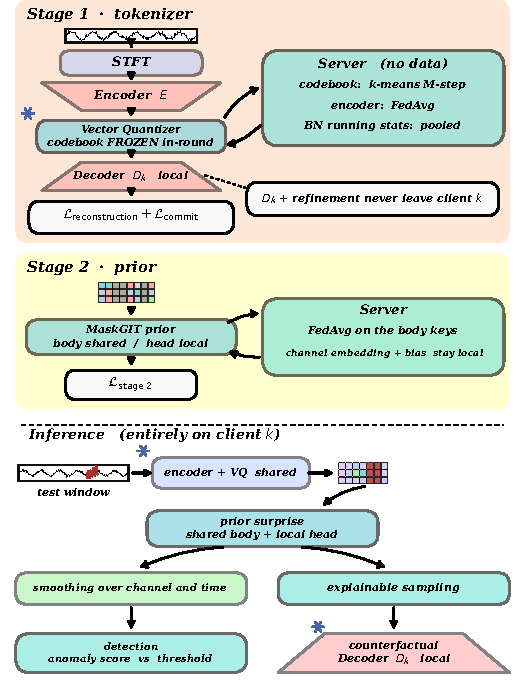
\includegraphics[width=\columnwidth]{fig_framework}
\caption{Configuration (g), the main federated arm, as it runs on client $k$. Stage~1 federates the
encoder and its BN running statistics and keeps the broadcast codebook fixed within a round, the
server updating it from assignment statistics as in~\eqref{eq:suffstat}; the decoder and the
refinement layer are never sent. Stage~2 shares the body of the MaskGIT prior and keeps the channel
embedding and the output bias local. Inference runs entirely on the client and forks: the prior's
surprise over the tokens becomes the anomaly score, while resampling the tokens it holds responsible
and decoding them locally produces the counterfactual.}
\label{fig:framework}
\end{figure}

\subsection{Tokenizer federation}
\label{subsec:tokenizer}

The encoder can remain local or be shared through FedAvg~\cite{mcmahan2017federated},
\begin{equation}
    \bar{\phi} = \sum_j \omega_j \phi_j.
\end{equation}
When the encoder is federated, its BN running statistics are pooled as
\begin{equation}
    \bar{\mu} = \sum_j \omega_j \mu_j, \qquad
    \bar{v} = \sum_j \omega_j (v_j + \mu_j^2) - \bar{\mu}^2.
\end{equation}
This is the opposite of the FedBN prescription, which keeps batch-normalization layers entirely
local to absorb feature shift between clients~\cite{li2021fedbn}. Here the clients observe the
same sensor and regime and differ only in how much of the series they hold, so there is no feature
shift for a local BN layer to absorb, while a shared tokenizer requires that every client normalize
identically before quantization.

The codebook can also be federated in different ways. Direct FedAvg averages corresponding codewords after local training; because each client's quantizer updates its dictionary independently during the round, corresponding entries may drift apart before aggregation, and the averaged codeword need not lie near any of them. This is our motivation for the alternative below, not a demonstrated defect of averaging: Section~\ref{subsec:interaction} reports the two rules to be indistinguishable in aggregate, and to differ substantially from series to series.

Our main alternative keeps the broadcast codebook fixed during each local round and aggregates assignment statistics. For every code $k$, client $j$ sends its number of assignments $c_{j,k}$ and the sum $m_{j,k}$ of the corresponding pre-quantization encoder vectors. The server computes
\begin{equation}
    N = \sum_j c_j, \qquad
    M = \sum_j m_j, \qquad
    e_k = M_k / \tilde{N}_k,
    \label{eq:suffstat}
\end{equation}
where $\tilde{N}_k$ is a Laplace-smoothed count. Thus, each global codeword is updated from statistics accumulated across clients without transmitting latent samples or raw data.

Keeping the codebook fixed during a round does not freeze the tokenizer: the encoder continues to change, and therefore the mapping from windows to codebook indices can still evolve.

\subsection{Prior federation}
\label{subsec:coupling}

Prior federation requires a shared token vocabulary. The MaskGIT prior predicts codebook indices, so index $k$ must refer to the same codeword across clients. Averaging prior parameters learned with independent client dictionaries would instead combine parameters associated with unrelated symbols. We therefore allow prior sharing only when clients use a common codebook.

A common dictionary alone does not guarantee identical token assignments, because those assignments also depend on the encoder; Section~\ref{subsec:interaction} measures how far apart clients end up in each case. We therefore evaluate prior sharing both with local encoders and after encoder federation.

We compare a fully local prior with a partially shared one. In the latter, the transformer, token embedding, frequency and time embeddings, and readout are shared, while the channel component of the positional encoding and an additive output bias remain local. On the univariate data considered here, personalization therefore acts mainly through the output bias.

Stage~2 is normally aggregated after a fixed number of local epochs. We also evaluate a variant in which every client performs exactly $\tau$ optimizer steps between two aggregations.

\subsection{Evaluated configurations}
\label{subsec:configs}

Table~\ref{tab:space} summarizes the evaluated configurations. Local and centralized training provide the reference points. The remaining configurations isolate the effects of sharing the codebook, encoder, and prior.

Two matched comparisons are especially important. Configurations (c) and (e) differ only in prior sharing while the encoder remains local. Configurations (f) and (g) make the same comparison after encoder federation. These contrasts test whether the effect of prior sharing depends on tokenizer alignment.

The last two configurations are diagnostic only and are not federation-legal: each replaces one stage by its pooled counterpart, so that the two stages can be blamed separately. The pooled-tokenizer configuration trains stage~1 on pooled raw windows and federates stage~2; the pooled-prior configuration is its mirror image, keeping the federated stage~1 of (g) and fitting the prior on the pooled token grids. Together they bound how much of the remaining gap to centralized training is attributable to each stage.

Configurations (j)--(m) vary how the encoder is aggregated, holding the codebook and prior settings of (f) fixed: FedProx~\cite{li2020fedprox} adds a proximal term to the local objective, FedProto~\cite{tan2022fedproto} broadcasts per-code prototypes instead of averaging weights, and (m) shares only the starting point. They federate the same encoder parameters as (f) but keep the BN running statistics local, which is why (j) restates FedAvg under that regime: the block is matched internally, and its baseline is (j) and not (f).

\begin{table}[t]
\caption{Configurations evaluated in the experiments. ``FedAvg'' denotes count-weighted parameter averaging, ``pooled'' the aggregation of BN statistics, ``suff.\,stat.'' the codebook update of~\eqref{eq:suffstat}, and ``partial'' the shared prior with client-specific components kept local. Column $n$ gives the number of development series on which the configuration was run, and in parentheses its coverage of the four series that separate the arms at all (Section~\ref{subsec:discriminating}). The other six are at ceiling or at floor for every configuration, so a row at $4/4$ covers the whole informative subset whatever its $n$, and a row below it is incomplete regardless of how large its $n$ is.}
\label{tab:space}
\centering
\scriptsize
\setlength{\tabcolsep}{2.2pt}
\renewcommand{\arraystretch}{1.15}
\begin{tabular}{@{}p{2.2cm}lllllc@{}}
\hline
\textbf{Configuration} & \textbf{Encoder} & \textbf{BN} & \textbf{Codebook} & \textbf{Prior} & \textbf{Stage 2} & $n$ (disc.) \\
\hline
(a) local & local & --- & local & local & --- & 10 (4/4) \\
(b) centralized & \multicolumn{5}{c}{one model on the pooled windows (reference)} & 10 (4/4) \\
\hline
(c) codebook only & local & --- & suff.\,stat. & local & --- & 10 (4/4) \\
(d) codebook only, averaged dictionary & local & --- & FedAvg & local & --- & 10 (4/4) \\
(e) codebook and shared prior body & local & --- & suff.\,stat. & partial & epochs & 10 (4/4) \\
(f) aligned tokenizer, local prior (A1) & FedAvg & pooled & suff.\,stat. & local & --- & 10 (4/4) \\
(g) aligned tokenizer, shared prior body (A2) & FedAvg & pooled & suff.\,stat. & partial & epochs & 10 (4/4) \\
(h) (g) with a step-counted rhythm & FedAvg & pooled & suff.\,stat. & partial & $\tau$ steps & 10 (4/4) \\
(i) (h) with a mobile dictionary & FedAvg & pooled & FedAvg & partial & $\tau$ steps & 3 (3/4) \\
\hline
\multicolumn{7}{@{}l@{}}{\emph{Encoder aggregation rule, isolated at a local prior}$^{\mathrm{c}}$} \\
(j) encoder FedAvg, local BN stats & FedAvg & affine & suff.\,stat. & local & --- & 10 (4/4) \\
(k) (j) with FedProx & FedProx & affine & suff.\,stat. & local & --- & 10 (4/4) \\
(l) (j) with FedProto & prototypes & init & suff.\,stat. & local & --- & 10 (4/4) \\
(m) (j) with a shared initialization only & init & init & suff.\,stat. & local & --- & 10 (4/4) \\
\hline
(n) score fusion$^{\mathrm{a}}$ & local & --- & local & local & --- & 10 (4/4) \\
\hline
\emph{pooled tokenizer}$^{\mathrm{b}}$ & \multicolumn{5}{c}{\emph{pooled stage 1, federated stage 2}} & 1 (1/4) \\
\emph{pooled prior}$^{\mathrm{b}}$ & \multicolumn{5}{c}{\emph{federated stage 1 of (g), stage 2 on pooled tokens}} & 4 (4/4) \\
\hline
\multicolumn{7}{@{}p{7.4cm}@{}}{$^{\mathrm{a}}$Trained exactly as (a); only inference differs, see Section~\ref{subsec:fusion}. $^{\mathrm{b}}$Not federation-legal because one stage sees pooled data; diagnostic only. The \emph{pooled prior} row is run on exactly the four discriminating series: the remaining six admit no movement for any arm, so its $n=4$ is a complete cover of the informative subset and not a shortfall. $^{\mathrm{c}}$Rows (j)--(m) federate the same $87$ encoder parameters as (f) but keep the BN running statistics local, so they are matched to one another and \emph{not} to (f)--(h): ``affine'' shares the BN scale and shift every round, ``init'' only at initialization. The local prior is a property of the block, which varies the aggregation rule alone; the corresponding rows with a shared prior are not evaluated, and Section~\ref{subsec:interaction} states what bounds them. FedProx uses $\mu=0.01$; (m) is (l) with the prototype pull set to zero, so it shares nothing after round~0.}
\end{tabular}
\end{table}

\subsection{Score fusion}
\label{subsec:fusion}

As an alternative to parameter sharing, we also combine independently trained local models at inference time. Each client keeps its tokenizer and prior unchanged and computes its anomaly-score profile $a_{\mathrm{final}}$. Each profile is standardized over time, and the final score is the pointwise mean across clients.

This avoids the need to align model parameters, codewords, or token indices: only per-timestep score vectors are combined. We use the mean of standardized scores as the default rule and report the median, trimmed mean, and mean of normalized ranks as alternative rules; Section~\ref{subsec:failure} shows the outcome is not stable across them. The procedure is offline and assumes that all client models score the same test series.

\section{Experimental Protocol}
\label{sec:protocol}

\subsection{Benchmark and choice of series}

We evaluate on the UCR Time Series Anomaly archive~\cite{wu2023ucr}. Following the configuration described in Section~\ref{sec:background}, each series uses window length $T=2P$, where $P$ is its manually measured period. This leaves 180 usable series: the remainder either have no measured period or leave the smallest client with fewer samples than one window.

The 180 series are used in two disjoint roles. Ten form a development set on which the federation configurations were explored. They were selected so that the period-aligned window length is approximately logarithmically spaced from $182$ to $970$ samples while covering different domains: four electrocardiograms, two respiration recordings, two arterial-pressure recordings, one cetacean acoustic recording, and one gait recording. Selection was therefore based on period and domain, not on anomaly-detection performance.

A second, disjoint set of 50 series was drawn uniformly at random, with a fixed seed, from the remaining 170. The same draw fixed their execution order. The sample, its order, the three configurations evaluated on it, the primary metric, the stopping rule, a minimum sample size, and a freeze date were fixed before observing results on these series. The development set is used for exploration; this random sample is reserved for confirmation and is analyzed in Section~\ref{subsec:confirmation}.

\subsection{Federated split}
\label{subsec:split}

\begin{figure*}[t]
\centering
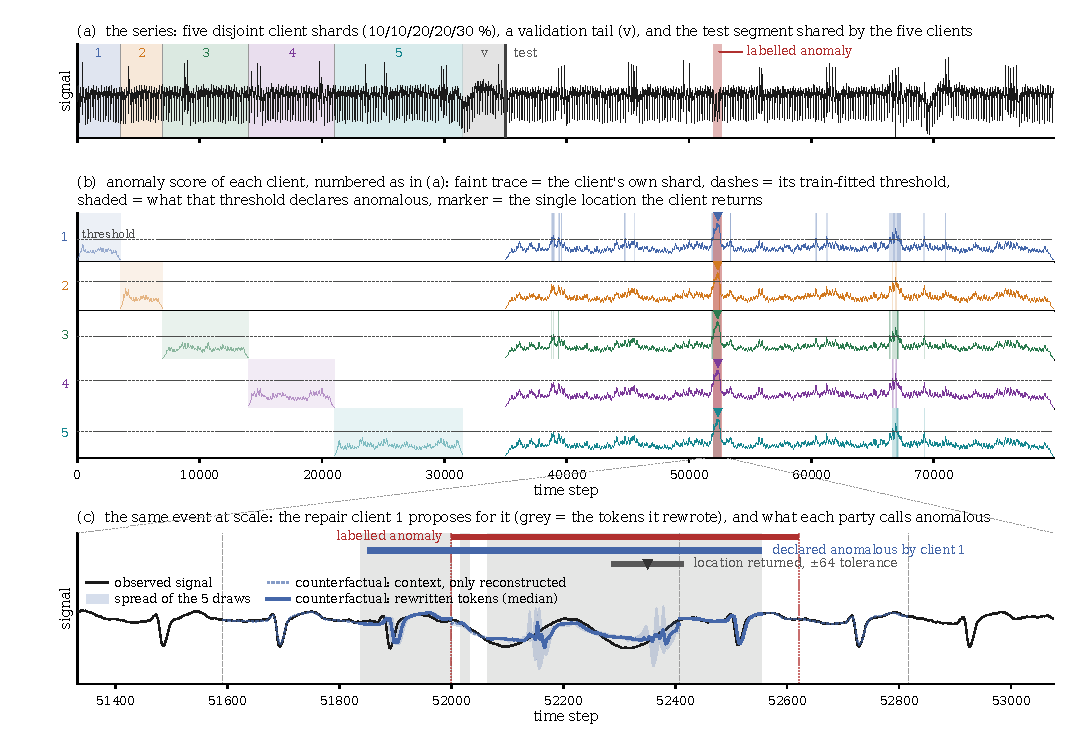
\includegraphics[width=\textwidth]{fig_overview}
\caption{One development series, \texttt{ucr\_001}, from the split to the explanation under
configuration (g). (a)~the series: its training segment is cut chronologically into five disjoint
client shards of $10/10/20/20/30\%$ followed by the validation tail (v), while the test segment and
its labels are shared by the five clients and never seen in training. (b)~the per-timestep anomaly
score of each client over the same time axis; the faint trace on the left is the same client scoring
its own shard, the dashed line is the threshold the original method fits on that shard alone, the
tinted bands are the timesteps it declares anomalous, and the marker is the single location the
client returns under the archive protocol. All five return the same location, inside the labelled
event, while their thresholds admit between $1.2\%$ and $4.1\%$ of the test timesteps: detection is
shared, but the decision each client would deploy is its own. (c)~that event at scale, with the
explanation as the original method builds it and \emph{no label in the loop}: the timesteps above
the client's own threshold are masked across the frequency dimension, resampled from the prior with
the remaining tokens frozen as context, and decoded locally. The grey spans are what client~1
rewrote, the band is the spread of five draws and the solid curve their median, while the dashed
curve is the same decoder passing through context it did not rewrite, and is reconstruction rather
than repair. On the window centred on the event the mask reaches the original method's cap of $90\%$
masked, which exists to leave the prior some context to condition on.
Section~\ref{subsec:counterfactual} instead masks the labelled positions, which is what keeps $|M|$
identical across configurations and the comparison paired. Every configuration already localizes
this series, so nothing here is a claim about the configurations; those are in
Section~\ref{sec:results}.}
\label{fig:overview}
\end{figure*}

Each series defines an independent federated task: no parameter, statistic, or window is shared between different series.

Within each series, the training segment is divided chronologically among five clients holding $10\%$, $10\%$, $20\%$, $20\%$, and $30\%$ of the data. The final $10\%$ is held out for validation. The archive's test segment and labels remain untouched and are never used during training. Figure~\ref{fig:overview} shows the arrangement on one series, together with the two outputs it produces: a score profile per client on the shared test segment, and the counterfactual analyzed in Section~\ref{subsec:counterfactual}.

Windows are extracted with unit stride. A client shard of length $L$ therefore contributes $L-T+1$ windows, and these counts determine the aggregation weights used in Section~\ref{sec:design}.

The split is deliberately homogeneous. All five clients observe the same sensor, regime, and units; they differ in how much of the series they hold rather than in the underlying task. This removes client distribution heterogeneity as the intended explanation for differences between local and federated training.

\subsection{Training}

All configurations use the same trainer and select the parameters of the best validation round, but the stopping criterion is granular to the setting and the two forms are not interchangeable. Local and centralized training stop on validation patience counted in optimizer steps, inside a fixed step budget; federated configurations stop on patience counted in aggregation rounds, since validation is only defined once per round. A federated run that exhausts its round ceiling without triggering patience is marked truncated and excluded. The step budget of the baselines is not exempt from the same concern: it binds in $9\%$ of the baseline stage-runs on the development set and in $15$--$25\%$ on the confirmation sample, where training ends with the budget rather than with the patience. Those runs are retained, so the baselines are, if anything, the arm more likely to be reported before convergence.

Model capacity is fixed across configurations. We use a codebook of $K=64$ entries of dimension $64$, an encoder with base width $16$, and a four-layer prior with four attention heads and width $128$, optimized with AdamW. The codebook is smaller than in the original method, so our reference results are not directly comparable with its published accuracy. One seed is run per experimental cell.

To calibrate what these numbers are worth, we also report a parameter-free floor: the squared residual of a centered moving average of length $10$, pushed through the same detection path as every deep configuration, with the same window geometry, impulse term~\eqref{eq:afinal}, and train-only threshold. Having no parameters, it admits no federated variant and is identical for every client, so it is a lower reference rather than a competitor.

\subsection{Metrics and unit of analysis}

We report the archive's accuracy and the area under the precision-recall curve (AUPRC) of the per-timestep anomaly score. For the archive metric, a method returns one predicted location per series and is counted as correct when it falls within $64$ timesteps of the labelled anomaly.

The two are chosen for different reasons and are not interchangeable. The archive metric is the
benchmark's own, so it leaves us no discretion and keeps the numbers comparable with the archive's
literature; it is correspondingly coarse, being a single hit or miss per series. AUPRC is ours, and
is there because it uses the whole per-timestep profile and therefore has the resolution the first
lacks. We do not report AUROC: with anomalies covering a small fraction of the timesteps it
saturates, and on the confirmation sample its median over the arms spans $0.947$ to $0.988$ against
$0.266$ to $0.473$ for AUPRC, while on eight of forty-eight series it exceeds $0.95$ for a
configuration whose predicted location misses the anomaly entirely. Threshold-based scores are
excluded for a related reason: the train-fitted threshold of the original method admits between
$0.000$ and $0.978$ of the test timesteps depending on the configuration, so it is not a comparable
currency across arms. Range-aware measures~\cite{paparrizos2022vus} are likewise not reported,
because their scale depends on anomaly duration and they are therefore not aggregable across
series. We do report the mean pairwise correlation between clients' standardized score profiles, as
a diagnostic of agreement between local models.

The unit of analysis is the series. The five clients are shards of one signal rather than independent replicates, so $n$ always denotes the number of series. Comparisons between configurations are paired by series.

Not every series can separate the methods. If local training already scores one, no method can improve it; if both local and centralized training score zero, the series provides no evidence about whether federation closes the collaboration gap. We identify such cases using the reference configurations alone and report comparisons both over all series and over the remaining discriminating series.

\section{Results}
\label{sec:results}

All results below are from the ten-series development set and use one seed per experimental cell. Client-level results are reduced to one value per series by averaging over the five clients. The same local baseline is used throughout; where a second, longer-budget run exists, it is reported only as a robustness check.

\subsection{Which series can separate the methods}
\label{subsec:discriminating}

The reference configurations divide the ten development series into three groups. On \texttt{ucr\_001}, \texttt{ucr\_083}, and \texttt{ucr\_086}, local training already obtains an archive score of $1.00$, leaving no room for improvement. On \texttt{ucr\_082}, \texttt{ucr\_222}, and \texttt{ucr\_229}, both local and centralized training score $0.00$.

The remaining four series---\texttt{ucr\_011}, \texttt{ucr\_014}, \texttt{ucr\_043}, and \texttt{ucr\_170}---can distinguish the configurations and are therefore the informative cases for the archive metric.

With only four discriminating series, a sign test cannot reach $p<0.05$: its minimum attainable value is $0.0625$. We therefore emphasize per-series magnitudes and win/loss counts rather than significance claims.

\subsection{Reference points}
\label{subsec:reference}

Pooling all client windows improves over the average local model on nine of ten series in AUPRC and on all four discriminating series in the archive metric. On these four series, local training obtains $0.40$, $0.80$, $0.20$, and $0.20$, whereas centralized training reaches $1.00$ in every case.

The comparison with the best individual client is different. Centralized training exceeds the best client on seven of ten series in AUPRC ($p=0.17$), but on the archive metric it never detects an anomaly that no individual client detects: centralized training and the best local client have identical scores on all ten series. Note that $\max_j$ is an oracle: selecting that client requires the test labels, so it bounds the achievable rather than naming a deployable choice.

Pooling therefore improves performance relative to a typical client without exceeding the strongest client on the archive metric.

The parameter-free floor stays far below all of them. Its median AUPRC over the ten series is $0.007$, against $0.353$ for local and $0.899$ for centralized training, and local, centralized, and federated training each exceed it on all ten series, although on \texttt{ucr\_082} every value is indistinguishable from zero. One series qualifies this: on \texttt{ucr\_083} the floor alone reaches $0.825$, so what that series measures is largely available without any learned model, which is consistent with its being uninformative about federation. The floor operates on the raw series and therefore does not apply the per-window z-normalization the detector inherits from the original method; the comparison crosses that boundary, but in the direction that makes it conservative, since the floor retains level and amplitude information that z-normalization removes from the deep models. Because its threshold falls back to a quantile rule, only threshold-free metrics are reported for it.

\subsection{Main federated configuration}
\label{subsec:main}

Configuration (g) of Table~\ref{tab:space} combines encoder FedAvg, pooled BN statistics, sufficient-statistics codebook aggregation, and a partially shared prior. It reaches the centralized archive score on three of the four discriminating series and fails on the fourth.

On \texttt{ucr\_011}, the archive score increases from $0.40$ under local training to $1.00$; on \texttt{ucr\_014}, from $0.80$ to $1.00$; and on \texttt{ucr\_043}, from $0.20$ to $1.00$. On \texttt{ucr\_170}, it instead falls from $0.20$ to $0.00$.

Across all ten series, this gives three improvements, one degradation, and six ties, with all six ties occurring on the non-discriminating series. In AUPRC, federation improves nine series and degrades one. The largest gains are concentrated on three series ($+0.42$, $+0.46$, and $+0.30$), while six of the improvements are below $0.035$.

Against centralized training, the federated model reaches the same archive score on nine of ten series and falls below it only on \texttt{ucr\_170}. In AUPRC it remains below centralized training on eight of ten series, showing that equal anomaly localization does not imply equal ranking of the full score profile.

The comparison with local training depends on where local training is stopped. Against the baseline used throughout, which stops on validation patience, federation improves nine of ten series in AUPRC (sign test $p=0.021$). Against a local baseline trained to a budget four to five times larger with early stopping disabled, the median difference is unchanged at $+0.022$ but the count falls to six wins and four losses ($p=0.75$): the longer-trained baseline is not uniformly better, it is more variable across series. The defensible claim is therefore that federation improves local training stopped at its own criterion, not that it improves local training at any budget.

\begin{table}[t]
\caption{Development set, ten series. Left: archive accuracy using one predicted location per series and a tolerance of $64$ timesteps. Right: AUPRC of the per-timestep anomaly score, with the parameter-free floor as the leftmost reference. $\max_j$ denotes the best individual local client and requires test labels to select. The four discriminating series are shown above the horizontal rule.}
\label{tab:main}
\centering
\scriptsize
\setlength{\tabcolsep}{2.2pt}
\renewcommand{\arraystretch}{1.1}
\begin{tabular}{@{}l cccc c ccccc@{}}
\hline
& \multicolumn{4}{c}{\textbf{accuracy@64}} & & \multicolumn{5}{c}{\textbf{AUPRC}} \\
\cline{2-5}\cline{7-11}
\textbf{series} & local & $\max_j$ & centr. & (g) & & floor & local & $\max_j$ & centr. & (g) \\
\hline
\texttt{ucr\_011} & 0.40 & 1.00 & 1.00 & \textbf{1.00} & & 0.092 & 0.403 & 0.997 & 0.976 & 0.820 \\
\texttt{ucr\_014} & 0.80 & 1.00 & 1.00 & \textbf{1.00} & & 0.003 & 0.639 & 0.902 & 0.964 & 0.939 \\
\texttt{ucr\_043} & 0.20 & 1.00 & 1.00 & \textbf{1.00} & & 0.046 & 0.181 & 0.819 & 0.875 & 0.637 \\
\texttt{ucr\_170} & 0.20 & 1.00 & 1.00 & 0.00 & & 0.015 & 0.303 & 0.588 & 0.878 & 0.086 \\
\hline
\texttt{ucr\_001} & 1.00 & 1.00 & 1.00 & 1.00 & & 0.007 & 0.820 & 0.903 & 0.920 & 0.851 \\
\texttt{ucr\_083} & 1.00 & 1.00 & 1.00 & 1.00 & & 0.825 & 0.922 & 0.983 & 0.932 & 0.932 \\
\texttt{ucr\_086} & 1.00 & 1.00 & 1.00 & 1.00 & & 0.007 & 0.938 & 0.979 & 0.986 & 0.973 \\
\texttt{ucr\_082} & 0.00 & 0.00 & 0.00 & 0.00 & & 0.000 & 0.000 & 0.000 & 0.000 & 0.000 \\
\texttt{ucr\_222} & 0.00 & 0.00 & 0.00 & 0.00 & & 0.002 & 0.046 & 0.077 & 0.083 & 0.054 \\
\texttt{ucr\_229} & 0.00 & 0.00 & 0.00 & 0.00 & & 0.002 & 0.002 & 0.003 & 0.018 & 0.005 \\
\hline
\end{tabular}
\end{table}

\subsection{Where the improvement comes from}
\label{subsec:interaction}

To isolate the effect of prior sharing, we apply the same modification under two tokenizer configurations. With a shared codebook but local encoders, configurations (c) and (e) differ only in whether the prior body is shared. With an aligned tokenizer, configurations (f) and (g) make the corresponding comparison after encoder federation. The set of shared prior tensors is identical in the two comparisons: $55$ keys are shared, while the channel embedding and output bias remain local.

With the aligned tokenizer, prior sharing improves nine of ten series in AUPRC, with median change $+0.069$, and all four discriminating series in the archive metric. With local encoders, the same modification gives four AUPRC improvements and six degradations, with median change $-0.001$, and splits two against two on the archive metric.

The difference between these effects is positive on eight of ten series in AUPRC, with median $+0.136$, and on all five non-tied series in the archive metric. In these experiments, prior sharing is therefore beneficial only after encoder alignment.

``Alignment'' is not a label we attach to the federated arm: it is a property of the checkpoints,
and it can be read off them. We encode the same validation windows with each client and measure how
often two clients assign the same latent position to the same code, corrected for the agreement
their marginal usage would produce by chance. Under (g) the five clients tokenize \emph{identically}
-- $\kappa=1.00$ on every one of the ten series -- whereas under (e), whose encoders are local, the
median is $\kappa=0.07$. The codebook is bit-identical across clients in both arms, so what
separates them is not the vocabulary but whether they use it the same way, which is exactly the
condition a prior indexed by code identity requires. The interaction of Table~\ref{tab:ablation} is
therefore not an unexplained contrast between two arms: it tracks a measured quantity that differs
by an order of magnitude between them.

The same measurement locates the intermediate mechanisms. Encoder FedAvg alone reaches
$\kappa=0.77$ under the BN regime of (j); pooling the BN running statistics, which is the only
remaining difference, carries it to $1.00$. Configuration (m), which shares the initialization and
never averages again, sits at $\kappa=0.04$, indistinguishable from the local encoders of (e) at
$0.07$ -- a common starting point does not survive local training. Federating the encoder does not
make the tokenizers better; it makes them agree.

Configurations (j)--(m) hold the prior local, so they do not establish whether a weaker alignment mechanism than encoder FedAvg would also support a shared prior. That question is bounded rather than open: (e) and (g) are the two extremes of the encoder axis \emph{with} the prior shared, and the whole effect lies between them. Of the three alternatives, FedProx still averages the encoder weights at the server -- its proximal term acts on the local objective only -- while FedProto and (m) never average them, so the first belongs structurally with (g) and the other two with (e). Where the intermediate mechanisms actually land is not measured here.

A shared prior with independent client dictionaries is not evaluated because the prior embedding is indexed by code identity; without a common vocabulary, averaging these parameters would combine unrelated token semantics.

What is shared therefore matters more than how it is averaged. Configurations (k), (l) and (m) replace encoder FedAvg by FedProx, by FedProto, and by a control that shares only the initialization, and none changes anything measurable: relative to (j), the same FedAvg under the same BN regime, the median AUPRC differences over the ten series are $-0.004$ ($3$ wins), $-0.004$ ($4$ wins), and $-0.000$ ($4$ wins). That the initialization-only control is indistinguishable from both algorithms is the strongest form of this null. Two qualifications apply: the block keeps the BN running statistics local, so its baseline is (j) and its values do not transfer numerically to (f)--(g) in Table~\ref{tab:main}; and FedProx uses $\mu=0.01$, whose proximal gradient falls below the solver's own detectability threshold on three of the ten series, where it is a no-op rather than a null.

The same holds for the codebook, with one difference worth stating. Configurations (c) and (d)
vary only how the dictionary is aggregated---sufficient statistics against direct averaging of the
codewords---with local encoders and local priors on both sides. In aggregate the two are
indistinguishable: five wins each over the ten series, median $-0.000$ AUPRC, and on the archive
metric three wins against two with five ties. They are not, however, interchangeable. The
per-series differences run from $-0.292$ to $+0.946$, and the largest of them is not a gain: on
\texttt{ucr\_083}, where the parameter-free floor alone reaches $0.825$, configuration~(c)
collapses to $0.005$ while (d) obtains $0.952$.

The same contrast after encoder alignment reproduces that shape on the three series where it was
run. Configurations (h) and (i) differ in the codebook rule and in nothing else, the stage-2
schedule included: direct averaging loses $0.063$ and $0.375$ AUPRC on \texttt{ucr\_011} and
\texttt{ucr\_043}---on the latter the archive accuracy falls with it from $1.00$ to $0.60$---and
gains $0.270$ on \texttt{ucr\_170}, the one series on which the frozen dictionary is the binding
constraint. Where the encoder rule was a null of small differences, the codebook rule is a null of
large ones that cancel, in both regimes: it is a source of per-series variance rather than a
systematic effect, and the variance is an order of magnitude larger than anything the encoder rule
produces. We therefore fix it to sufficient statistics throughout and do not present that choice as
a contribution.

One limitation affects this comparison. The aligned and unaligned branches were not run entirely on matched hardware: configuration (g) ran on one accelerator, whereas configuration (e) used two other accelerators for seven of the ten series. This difference is therefore a potential confound that cannot be separated with the available runs.

\begin{table}[t]
\caption{Effect of prior sharing with and without encoder alignment. $d_A=(g)-(f)$ compares shared and local priors with an aligned tokenizer; $d_F=(e)-(c)$ makes the same comparison with local encoders. W/L/T denote wins, losses, and exact ties over the ten series.}
\label{tab:ablation}
\centering
\scriptsize
\setlength{\tabcolsep}{4pt}
\renewcommand{\arraystretch}{1.1}
\begin{tabular}{@{}l cc cc@{}}
\hline
& \multicolumn{2}{c}{\textbf{AUPRC}} & \multicolumn{2}{c}{\textbf{accuracy@64}} \\
\cline{2-3}\cline{4-5}
\textbf{contrast} & W/L/T & median & W/L/T & median \\
\hline
$d_A$ (aligned tokenizer) & 9/1/0 & $+0.069$ & 4/0/6 & $+0.00$ \\
$d_F$ (local encoders) & 4/6/0 & $-0.001$ & 2/2/6 & $+0.00$ \\
\hline
$d_A-d_F$ (interaction) & 8/2/0 & $+0.136$ & 5/0/5 & $+0.20$ \\
\hline
\end{tabular}
\end{table}

\subsection{Stage-2 synchronization}
\label{subsec:stage2}

Two stage~2 choices were varied on the full development set while reusing the same stage~1 checkpoint, so that the tokenizer is identical within each comparison.

Fixing the validation masks and evaluating in single precision removes mask-resampling noise from round selection. This improves five series and degrades four, with the largest gains on \texttt{ucr\_043} ($+0.109$ AUPRC) and \texttt{ucr\_011} ($+0.049$).

Replacing epoch-based rounds with $\tau=64$ optimizer steps improves four series and degrades six, with median change $-0.001$. Increasing synchronization frequency beyond the default therefore provides no measurable benefit on this development set.

A run with a comparable step budget but less frequent aggregation---approximately $310$ local steps between server updates instead of $100$--$190$---loses $0.198$ AUPRC on \texttt{ucr\_011} and $0.245$ on \texttt{ucr\_043}. The default synchronization frequency therefore appears sufficient, while substantially less frequent aggregation can degrade performance.

This null holds out of sample. Configuration (h) was also run on all forty-eight series analyzed in
Section~\ref{subsec:confirmation}, resuming from the bit-identical stage~1 of (g) so that only
stage~2 differs, and every one of the forty-eight cells converged. Against (g) on the same shards
it wins twenty-five series and loses twenty-three in AUPRC, with median difference $0.0000$ and
mean $+0.006$ ($p=0.89$); on the archive metric it wins two, loses four, and ties forty-two
($p=0.69$). The largest differences run in both directions, $+0.186$ on \texttt{ucr\_106} against
$-0.145$ on \texttt{ucr\_250}. One qualification: (h) bundles the fixed validation masks with the
step-counted rhythm, so this contrast bounds the pair rather than isolating $\tau$, the two having
been separated only on the development set. What it establishes is that the stage-2 schedule, tuned
as far as we tuned it, buys nothing on a random sample five times larger than the set on which it
was tuned.

\subsection{Failure case and score fusion}
\label{subsec:failure}

\texttt{ucr\_170} is the only discriminating series on which the main federated configuration fails to recover the local baseline. The five local models obtain AUPRC values of $0.004$, $0.223$, $0.329$, $0.588$, and $0.370$, with mean pairwise score-profile correlation $0.56$. After federation, the corresponding values become $0.087$, $0.094$, $0.088$, $0.073$, and $0.088$, while correlation increases to $0.98$. The clients therefore become substantially more similar, but the common profile ranks a false alarm above the true anomaly. The centralized model contains the same false-alarm region but ranks it below the anomaly.

The two diagnostic configurations locate the responsibility. Replacing only the prior of (g) by one fitted on the pooled token grids raises AUPRC to $0.948$, $0.947$, $0.900$, and $0.202$ on the four discriminating series, against $0.870$, $0.944$, $0.746$, and $0.082$ for the matched federated reference: an improvement on all four, but one that reaches the centralized level on the first three and not on \texttt{ucr\_170}. Conversely, replacing only the tokenizer by a pooled one recovers \texttt{ucr\_170} to $0.578$. On most series the federated tokenizer is therefore not the binding constraint and the prior is; on \texttt{ucr\_170} the order reverses. Both configurations see pooled data at one stage and are reported as bounds, not as methods; each rests on at most four series and a single seed.

Combining the original local models at the score level performs substantially better on this series. Averaging their standardized profiles gives AUPRC $0.698$, compared with $0.086$ for the weight-aggregated model trained on the same shards, and also above the best individual client at $0.588$: this is the only series in the development set on which the ensemble exceeds every model entering it. The gain depends on the combination rule and lives in the amplitude of the peaks rather than in their ordering: the trimmed mean obtains $0.690$, but the median and the mean of normalized ranks fall to $0.363$ and $0.277$. Applying the same fusion to the federated clients changes nothing ($0.087$ against $0.086$), because their profiles are already nearly identical.

The combination rule therefore matters. Across the rest of the development set, however, score fusion provides no comparable advantage, and applying it to the already federated models adds little because their outputs are nearly identical. We therefore treat score fusion as a repair for this failure mode rather than as the main detector.

\subsection{Confirmation on the random sample}
\label{subsec:confirmation}

Everything above was measured on the purposively chosen development set, which cannot estimate a
population. The pre-registered random sample of Section~\ref{sec:protocol} exists to test whether
the two claims that survive there also hold out of sample, and its analysis was fixed before any of
its numbers were produced: the primary endpoint is the archive accuracy at tolerance $64$, compared
between arms by a paired sign test across series with ties counted as ties, and AUPRC is secondary.
Three configurations are run on it: local, centralized, and (g).

Of the fifty series, forty-eight are analyzed. On two, \texttt{ucr\_190} and \texttt{ucr\_240},
the federated arm terminated with an assertion failure: the aggregated codebook contained
non-finite entries, which the broadcast-consistency check between the server and the clients
detects. The proximate cause is a non-finite latent entering the sufficient statistics
of~\eqref{eq:suffstat}, where a single non-finite coordinate propagates through the one-hot
reduction to almost every codeword; whether it originates in half-precision overflow or in a
diverging encoder is not determined by our logs, since neither run wrote a checkpoint. It is not
codebook collapse: on \texttt{ucr\_190} the perplexity had recovered from $2.6$ of $64$ codes at
round three to $10.8$ with no dead codes at round five, the round before the failure. The
pre-registered rule discards a series from \emph{all} arms when any arm is incomplete.

The missingness is not at random, but its consequence is bounded. Among the five series whose
encoder has an identical architecture, the encoder drift at round five increases monotonically with
the number of half-precision forward steps per round --- $1.39$, $1.58$, $3.03$, $3.60$ and $8.89$
at $3.5$k, $3.5$k, $6.1$k, $7.4$k and $9.1$k steps, the last being \texttt{ucr\_190} --- and
\texttt{ucr\_240} carries $31$k steps per round on the only deeper encoder in the sample. The
failure therefore tracks training exposure rather than detection difficulty. On the primary
endpoint both series sit at floor for the two reference arms, which score $0.00$ on each, and among
the thirteen analyzed series where local and centralized training both score zero the federated arm
is non-zero on one. Recovering both would be expected to add $0.15$ non-tied series, and even if
both were recovered as wins the primary contrast against local training would move only from
$p=0.33$ to $p=0.17$.

\begin{table}[t]
\caption{Confirmation sample, $n=48$ series, paired by series. The primary endpoint is the archive
accuracy at tolerance $64$; AUPRC is secondary and describes the direction of the effect. W/L/T are
wins, losses and ties; $p$ is a two-sided sign test with ties excluded from the test and counted in
the table. The mean is reported alongside the median because on the primary endpoint the median is
zero by construction wherever ties dominate.}
\label{tab:c50}
\centering
\scriptsize
\setlength{\tabcolsep}{4pt}
\renewcommand{\arraystretch}{1.1}
\begin{tabular}{@{}l cccc c ccc@{}}
\hline
& \multicolumn{4}{c}{\textbf{accuracy@64} (primary)} & & \multicolumn{3}{c}{\textbf{AUPRC} (secondary)} \\
\cline{2-5}\cline{7-9}
\textbf{contrast} & W/L/T & med. & mean & $p$ & & med. & mean & $p$ \\
\hline
(g) $-$ local          & 11/6/31 & 0.000 & $+0.083$ & 0.332 & & $+0.027$ & $+0.073$ & \textbf{0.029} \\
centralized $-$ local  & 14/5/29 & 0.000 & $+0.142$ & 0.064 & & $+0.053$ & $+0.141$ & \textbf{0.002} \\
(g) $-$ centralized    & 3/8/37  & 0.000 & $-0.058$ & 0.227 & & $-0.009$ & $-0.067$ & 0.060 \\
\hline
\end{tabular}
\end{table}

Reported in the fixed order, primary endpoint first: \emph{on the pre-registered primary endpoint
none of the three contrasts reaches $p<0.05$}. Configuration~(g) improves on local training on
eleven series and loses on six, with thirty-one ties ($p=0.33$); centralized training improves on
fourteen and loses on five ($p=0.06$); and (g) is below centralized training on eight series
against three ($p=0.23$). The confirmation, on the endpoint we committed to, does not confirm.

The reason is visible in the tie counts rather than in the effect. The archive metric scores one
predicted location per series and we average it over five clients, so a series contributes to the
test only when the arms disagree about whether that location is found; on this sample they agree on
thirty-one of forty-eight for the first contrast and thirty-seven of forty-eight for the third. The
effective sample size is therefore seventeen and eleven, not forty-eight, and no effect of the size
observed here could have reached significance on the third contrast at all. Where the arms do
differ, the direction is the one the development set predicted: the mean difference is $+0.083$ for
(g) over local training and $+0.142$ for centralized training over it.

This is a property of the endpoint and not of federation, and the pooled model is the evidence:
centralized training sees every client's data and still does not separate from local training on
this metric ($p=0.06$). No arm does. Read against that, the federated model's position on the
primary endpoint is parity with the pooled upper bound -- identical scores on thirty-seven of
forty-eight series -- reached without any client's windows leaving it. The endpoint we
pre-registered turns out to have too little resolution on this archive to confirm or refute a
difference of the size any of these methods produce, which is a fact about the metric that we could
not have known before fixing it, and which we report rather than replace after the fact.

On the secondary endpoint the picture is the one the development set showed, and it is significant:
in AUPRC, centralized training improves on local training on thirty-five of forty-eight series
($p=0.002$) and (g) on thirty-two of forty-eight ($p=0.029$), while (g) remains below centralized
training on thirty-one of forty-eight ($p=0.06$). The tension between the two metrics that
Section~\ref{subsec:discriminating} documents on ten purposively chosen series is therefore not an
artifact of that choice: it reproduces on a random sample five times larger. Out of sample, the
defensible statement is that federated and pooled training both improve the ranking of anomalous
timesteps over the typical client, and that neither is shown to improve the archive's own
localization accuracy.

\subsection{Counterfactual quality}
\label{subsec:counterfactual}

Everything above measures detection. The method also returns an explanation: the tokens it holds
responsible are masked, resampled from the prior with the remaining tokens frozen as context, and
decoded back to a waveform. The score never reaches the decoder, so the counterfactual is the only
output that passes through it, and the decoder is local in every configuration. Whether federation
costs anything on this second product is therefore a separate question.

The comparison is paired on the window and on the mask, so that only the model varies, and the mask
is derived from the labels: a model-driven selection would silently vary $|M|$ with the arm, since
the paper-style threshold admits between $0.000$ and $0.978$ of the test timesteps depending on the
configuration. For each of five series we take eight anomalous windows, sampled at constant stride
along the event and each retaining at least $10\%$ of normal context, and eight normal windows whose
$|M|$ matches the median of the anomalous ones. Plausibility is the relative gain
$\Delta = [\mathrm{NLL}(x)-\mathrm{NLL}(x_{\mathrm{cf}})]/\mathrm{NLL}(x)$ on the rewritten
positions, with $x_{\mathrm{cf}}$ re-encoded from the waveform; scoring the sampled tokens directly
would be circular. The round trip preserves only $38$--$65\%$ of them, so $\Delta$ measures what the
encoder reads back. Specificity is $G = \Delta(\text{anomalous}) - \Delta(\text{normal})$, which
controls for a generator that simply makes every input more typical.

Each arm is judged by its own prior, so $\Delta$ is a within-model quantity and its levels are not
comparable across arms; $G$ is, being a difference of two $\Delta$ values under the same prior.

\begin{table}[t]
\caption{Counterfactual quality. $\Delta$ is the plausibility gain on the rewritten positions, each
arm under its own prior; $G$ is the specificity gap between anomalous and normal windows. Rows above
the rule are the four series that separate the arms on detection; \texttt{ucr\_001} below it is at
ceiling for all three. No median row is given: the unit is the series, and the paired contrasts in
the text are the relevant comparison.}
\label{tab:cf}
\centering
\scriptsize
\setlength{\tabcolsep}{4pt}
\renewcommand{\arraystretch}{1.1}
\begin{tabular}{@{}l ccc c ccc@{}}
\hline
& \multicolumn{3}{c}{\textbf{$\Delta$ plausibility}}
& & \multicolumn{3}{c}{\textbf{$G$ specificity}} \\
\cline{2-4}\cline{6-8}
\textbf{series} & local & centr. & (g) & & local & centr. & (g) \\
\hline
\texttt{ucr\_011} & 0.541 & 0.577 & 0.588 & & 0.289 & 0.609 & 0.403 \\
\texttt{ucr\_014} & 0.411 & 0.542 & 0.600 & & 0.232 & 0.263 & 0.270 \\
\texttt{ucr\_043} & 0.264 & 0.166 & 0.232 & & 0.083 & 0.110 & 0.213 \\
\texttt{ucr\_170} & 0.415 & 0.559 & 0.225 & & 0.406 & 0.685 & 0.553 \\
\hline
\texttt{ucr\_001} & 0.286 & 0.208 & 0.295 & & 0.073 & $-0.015$ & 0.118 \\
\hline
\end{tabular}
\end{table}

Table~\ref{tab:cf} collects the results. Every arm rewrites anomalies into content its own prior
finds more typical than what it replaced ($\Delta>0$ in all fifteen cells), and all but one pass the
specificity control ($G>0$ in fourteen of fifteen; the exception is centralized training on
\texttt{ucr\_001}, at $-0.015$). The repairs therefore appear targeted rather than the result of
uniform smoothing.

On the comparable quantity, federation does not lose. Specificity favors it over local training on
all five series, with median paired difference $+0.114$, and is level with centralized training, at
$+0.007$. Client agreement, measured as between-client MAE in units of each model's own sampling
noise, is likewise similar: median ratio $2.4$ for the federated clients against $2.2$ for the local
ones, the federated models disagreeing less in absolute terms but also sampling more
deterministically.

\begin{figure*}[t]
\centering
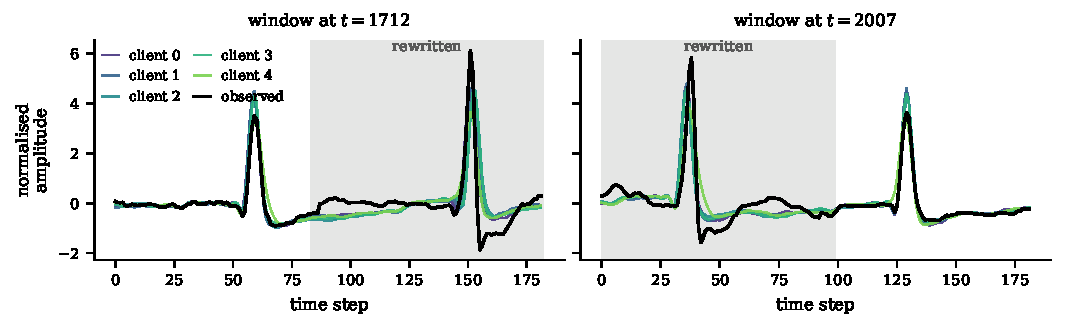
\includegraphics[width=\textwidth]{fig_counterfactual}
\caption{Counterfactuals from configuration (g) on \texttt{ucr\_011}, with all five clients shown.
The two panels show the same anomaly as the sliding window enters it from the right and leaves it
to the left. Shading marks the rewritten tokens; the mask is derived from the labels and is
therefore identical across clients and arms. Deviation outside the shaded span is reconstruction
error rather than rewriting. In both panels, the anomalous undershoot following the peak is
replaced by the flatter return observed elsewhere in the series.}
\label{fig:cf}
\end{figure*}

Figure~\ref{fig:cf} illustrates the resulting counterfactuals, with all five clients on one event:
they propose similar repairs, replacing the anomalous excursion by a motif observed elsewhere while
largely preserving the surrounding context. The masks there are the label-derived ones this section
measures, and are therefore narrower than the deployed rule illustrated in
Figure~\ref{fig:overview}(c), where the mask is whatever the client's own threshold declares.

This is a null result, not evidence of equivalence. Five series and a single seed provide limited
power, and UCR carries no counterfactual ground truth, so these metrics measure typicality and
targeting rather than correctness. Within those limits, federation shows no counterfactual-quality
loss comparable to the differences it produces in detection.

\subsection{Limitations}
\label{subsec:limitations}

Four limits bound what the above can support. Every cell is a single seed, so no error bar in
this section comes from repeated runs of the same configuration, and per-series differences
below a few hundredths should not be read as effects. Six of the ten development series cannot
separate the arms at all, leaving four informative comparisons and a sign test that cannot
reach $p<0.05$ on them by construction. The development set was chosen purposively -- by a
property of the series' period, not by difficulty or by how federation behaves on it -- so no
quantity measured on it estimates a population; that role belongs to the random sample of
Section~\ref{subsec:confirmation}, whose primary endpoint proved too coarse to separate any pair of
arms, so the confirmation rests on the secondary one. And the treated branch of
Section~\ref{subsec:interaction} is not matched on hardware, a confound we can declare but not
bound.

\section{Conclusion}
\label{sec:conclusion}

We asked what a federated learner should share when the detector is built from a discrete
tokenizer and a prior over the tokens it emits. The two stages turn out not to be separable
choices. Sharing the body of the prior improves detection only after the clients' encoders have
been averaged, and the identical modification is a null when they have not been. Alignment here is
not a label we attach to the federated arm but a quantity we read off the checkpoints: under the
strongest configuration the five clients tokenize \emph{identically}, $\kappa=1.00$ on every
development series, against a median of $0.07$ with local encoders --- with a bit-identical
codebook on both sides. What separates the two regimes is therefore not the vocabulary but whether
the clients use it the same way, which is precisely the condition a prior indexed by code identity
requires.

Within that constraint, \emph{what} is shared matters more than \emph{how} it is aggregated.
Replacing encoder FedAvg by FedProx, by FedProto, or by a control that shares only the
initialization changes nothing measurable, and the initialization-only control being
indistinguishable from both algorithms is the strongest form of that null. Changing the codebook
rule instead changes a great deal on individual series and nothing in aggregate. Both aggregation
axes are places where a designer has latitude; the choice of which components to share is not.

The empirical bottom line is deliberately narrow. On a random sample fixed in advance, the
federated model improves the ranking of anomalous timesteps over local training on thirty-two of
forty-eight series ($p=0.029$), and matches pooled training on the archive's own localization
metric on thirty-seven of forty-eight. On that metric our pre-registered primary endpoint separates
no pair of arms at all, pooled training included, so what the sample establishes is parity with an
upper bound that does not itself separate --- not a demonstrated gain in localization. We report
the endpoint as fixed rather than replace it after seeing the result.

Two further findings bound the picture. Weight-space aggregation can propagate one client's false
alarm to every client, and on the one series where it does, combining the local models' scores
instead of their weights recovers most of the gap at no training cost: the diversity an ensemble
exploits is exactly what parameter averaging destroys. And on the counterfactual the method also
produces, federation costs nothing we can measure, which locates its price entirely in detection.

\section{Future Work}
\label{sec:future}

Four directions follow directly from what these experiments could not settle.

The first is statistical. Every cell reported here is a single seed, so per-series differences below
a few hundredths carry no interpretation, and the effect sizes we do report have no error bar of
their own. Repeating the two matched contrasts of Section~\ref{subsec:interaction} across seeds is
the cheapest way to convert the interaction from a consistent direction into a quantity, and it is
the change that would strengthen the central claim most per unit of computation.

The second is the alignment axis itself. The encoder-aggregation block holds the prior local, so the
grid of aggregation rule against prior sharing is measured only at its two extremes: local encoders
with a shared prior, and full FedAvg with a shared prior. Our $\kappa$ measurements show that a
common initialization does not survive local training, but they leave open where partial mechanisms
land --- averaging only the deepest encoder layers, averaging every few rounds rather than every
round, or re-synchronizing only when a divergence statistic crosses a threshold. If any of these
reaches the alignment that prior sharing needs, the communication cost of the whole method drops
substantially.

The third is the endpoint. The archive's own accuracy metric proved too coarse to separate any pair
of arms on our confirmation sample, pooled training included, because a single hit or miss per
series produces ties wherever the arms agree. A confirmation designed around an endpoint with more
resolution, pre-registered with the same discipline, would test the claims this one could not; the
result reported in Section~\ref{subsec:confirmation} is as much a finding about the metric as about
the methods.

The fourth is the client model. Our split is deliberately homogeneous: five shards of one signal,
differing in quantity alone, so that heterogeneity is not available as an explanation. Real
deployments differ in sensor, calibration, and regime, and two of our design choices are expected to
invert there --- pooling the BN running statistics, which we adopt against the FedBN
prescription~\cite{li2021fedbn} precisely because no feature shift exists here, and a single shared
codebook, whose adequacy is an open question once clients observe genuinely different signals.
Finally, the two runs that ended on the confirmation sample failed because non-finite values reached
the aggregated codebook, which is a failure mode of federated vector quantization in its own right:
the sufficient-statistic aggregation of~\eqref{eq:suffstat} carries no finiteness guard, and one
non-finite coordinate in one client's statistics propagates to nearly every codeword. The
broadcast-consistency check makes this loud in the federated arms; local and centralized training
update the codebook without an equivalent check, so the same event would be silent there.

\section*{Data and Resources}
The data used in this study are in the \href{https://www.cs.ucr.edu/\%7Eeamonn/time_series_data_2018/UCR_TimeSeriesAnomalyDatasets2021.zip}{UCR Time Series Anomaly Archive}. The implementation of [NAME] is available on %\href{LINK}{LINK}.

\section*{Acknowledgment}

This work was supported by the MSCA Doctoral Networks project T.U.A.I. -- Towards an Understanding of Artificial Intelligence via a transparent, open and explainable perspective (TUAI), Grant Agreement No.~101168344.

% Pareggia le due colonne dell'ultima pagina: rompe la colonna prima della ref
% indicata (senza pacchetti, e' nativo IEEEtran). ⚠️ E' un indice HARD-CODED:
% si sfasa a ogni modifica del testo o della bibliografia. Va ritarato prima
% della submission: misurato oggi, 12 -> scarto 22pt (senza, 209pt).
\IEEEtriggeratref{12}
\bibliographystyle{IEEEtran}
\bibliography{references}

\end{document}
